\subsection{time-stretching}
\begin{frame}\frametitle{time stretching \& pitch shifting}\framesubtitle{introduction}
	\begin{itemize}
		\item	\textbf{time stretching}\\
			change playback speed/tempo without changing pitch
		\pause
        \bigskip
		\item	\textbf{pitch shifting}\\
			change pitch without changing tempo/playback speed
		\pause
        \bigskip
		\item	\textbf{terms}
            \begin{itemize}
                \item   time/pitch scaling
                \item   time expansion/compression
            \end{itemize}
	\end{itemize}

\end{frame}

\begin{frame}\frametitle{time stretching \& pitch shifting}\framesubtitle{applications}
	\begin{itemize}
		\item	\textbf{beat matching}: align tempo of two or more audio files (mashup)
		\pause
        \smallskip
		\item	\textbf{key lock}: ``align'' pitch of two or more audio files (mashup)
		\pause
        \smallskip
		\item	\textbf{pitch/time correction}: edit intonation, frequency deviation, vibrato, glissando
		\pause
        \smallskip
		\item	video \textbf{frame rate conversion}
		\pause
        \smallskip
		\item	\textbf{sample player/libraries}
		\pause
        \smallskip
		\item	\textbf{sound design}
		\pause
        \smallskip
		\item	\textbf{educational software}: pitch and timing visualization
	\end{itemize}
\end{frame}
\begin{frame}\frametitle{time stretching \& pitch shifting}\framesubtitle{stretch and pitch factors}
	\begin{eqnarray*}
		s	&=& \frac{t_{output}}{t_{input}}\\
		p	&=& \frac{f_{output}}{f_{input}}
	\end{eqnarray*}
	\pause
	\textbf{examples}:
	\begin{itemize}
		\item	\textit{half speed}: 
			\pause
			$s = 2$
		\pause
		\item	\textit{half pitch}: 
			\pause
			$p = \frac{1}{2}$
		\pause
		\item	\textit{semitone up/down}: 
			\pause
			\begin{equation}
				p_u = 2^{\nicefrac{1}{12}} = 1.059\quad p_d = 2^{-\nicefrac{1}{12}} = 0.9439\nonumber
			\end{equation}
		\pause
		\item	\textit{\unit[100]{BPM} $\rightarrow$ \unit[75]{BPM}}: 
			\pause
			$s = \frac{4}{3}$
	\end{itemize}
\end{frame}
    \begin{frame}{time stretching \& pitch shifting}{resampling}
        \begin{itemize}
            \item   \textbf{traditional}: resampling
                \begin{itemize}
                    \item   change inter-sample 'distance' by interpolation
                    \item   keep playback sample rate constant
                    \pause
                    \bigskip
                    \item   audio example
                    \uncover<2->{
                        \begin{itemize}
                            \item   original \includeaudio{audio/cathy.mp3}
                            \item   resample \includeaudio{audio/cathyResample.mp3}
                        \end{itemize}
                        }
                    \pause
                    \bigskip 
                    \item[$\Rightarrow$] tempo change results in pitch change (and vice versa)
                    \begin{equation*}
                        s = \frac{1}{p}
                    \end{equation*}
                \end{itemize}
        \end{itemize}
    \end{frame}
 
\begin{frame}\frametitle{time stretching \& pitch shifting}\framesubtitle{stretching: frequency domain}
		\begin{figure}
			\centerline{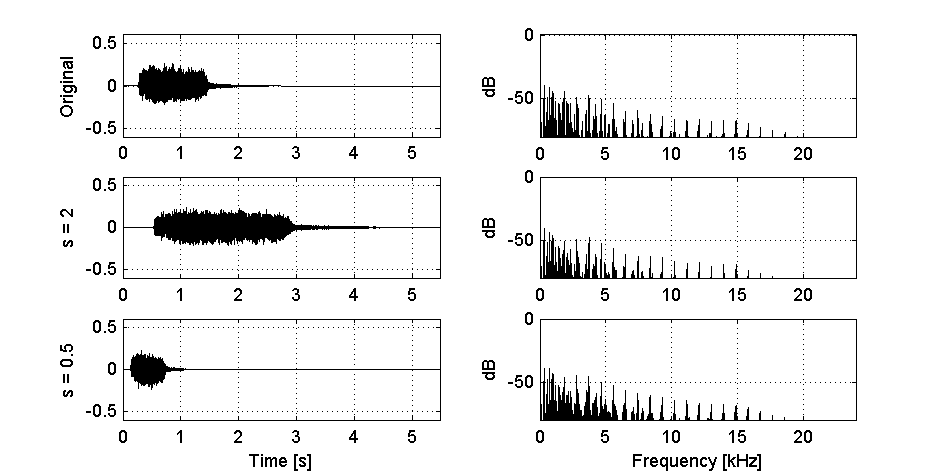
\includegraphics[scale=.7]{graph/fx4_timestretchintro}}
		\end{figure}
\end{frame}
   
    \subsection{time-segment processing (ola)}
    \begin{frame}{OLA}{introduction}
        overlap and add approaches for, e.g.,
        
        \begin{itemize}
            \item   granular synthesis
            \item   time/frequency synthesis and processing
            \item   {\color<2->{gtgold}time-stretching and pitch-shifting}
        \end{itemize}
    \end{frame}

    \begin{frame}{OLA}{time stretching}
            \textbf{overlap and add}
            \begin{enumerate}
                \item	\textbf{split input} signal into overlapping blocks
                \pause
                \item	\textbf{duplicate or discard blocks} depending on stretch factor
                %\item[] \includemovie[poster=graph/SpeakerIcon.png,mouse=true]{5mm}{5mm}{audio/cathyOLAout.mp3} $s = \nicefrac{4}{3}$
            \end{enumerate}
            \uncover<2->{
            \begin{columns}
                \column{6cm}\vspace{-5mm}
                    \begin{figure}
                        \centering
                        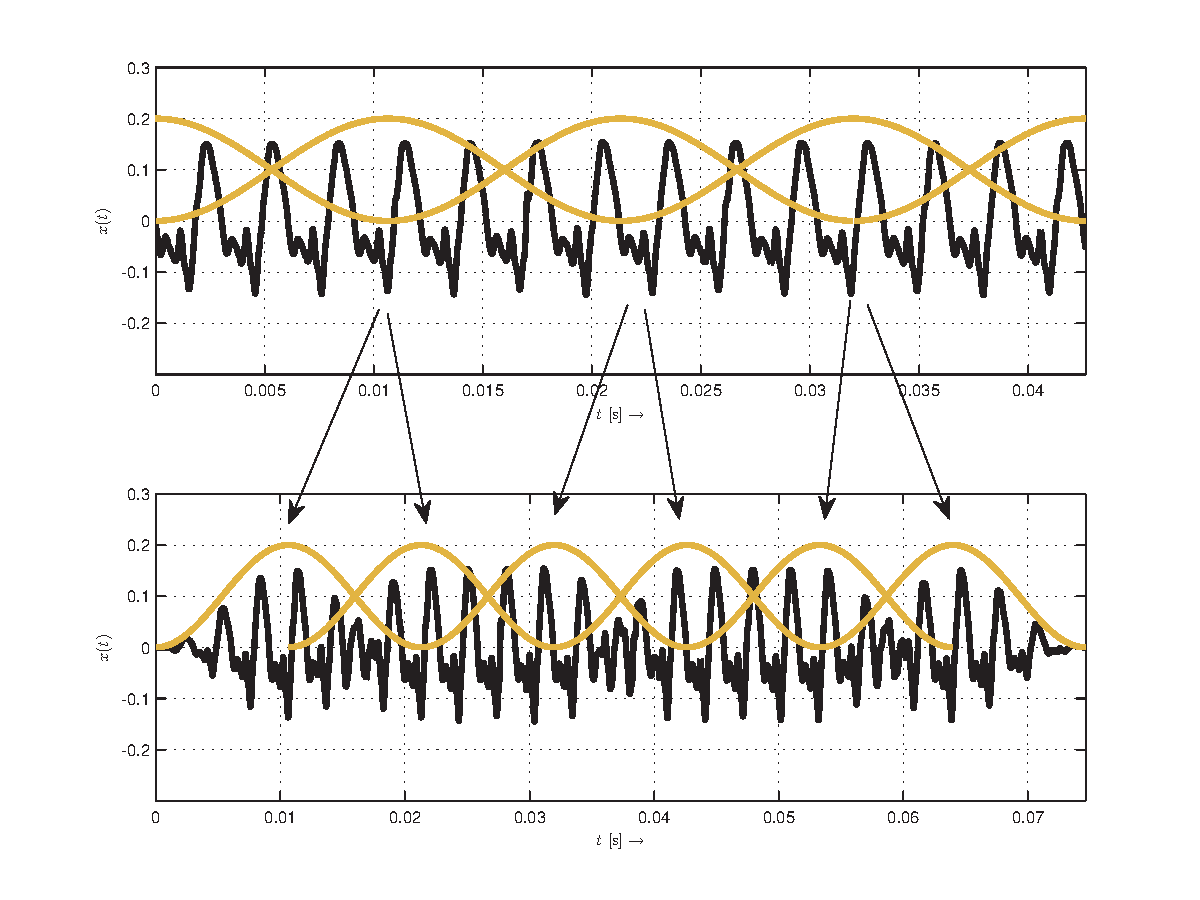
\includegraphics[scale=.3]{graph/OLA}
                    \end{figure}\vspace{-5mm}

                \column{4cm}\vspace{-20mm}
                    \begin{itemize}
                        \item orig  \includeaudio{audio/cathy.mp3}
                        \item $s = \nicefrac{4}{3}$ \includeaudio{audio/cathyOLAout.mp3}
                    \end{itemize}
            \end{columns}
            }
    \end{frame}

    \begin{frame}{PSOLA}{time stretching}
            \textbf{pitch synchronous overlap and add}
            \begin{itemize}
                \item   use the OLA principle, but
                \item	\textbf{adapt block length} to fundamental period length
            \end{itemize}
            \only<1>{
            \begin{figure}
                \centerline{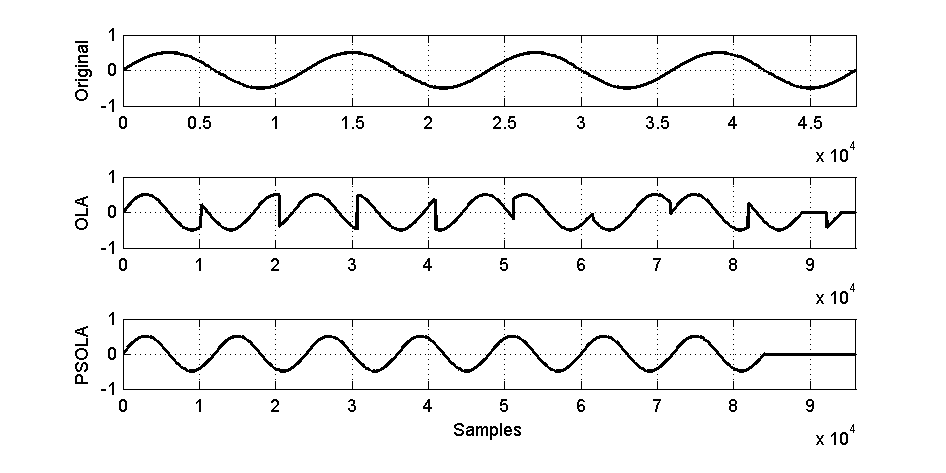
\includegraphics[scale=.6]{graph/fx4_olapsola}}
                \label{fig:fx4_olapsola}
            \end{figure}
            }          
            \pause
            \begin{columns}
                \column{6cm}\vspace{-5mm}
                    \begin{figure}
                        \centering
                        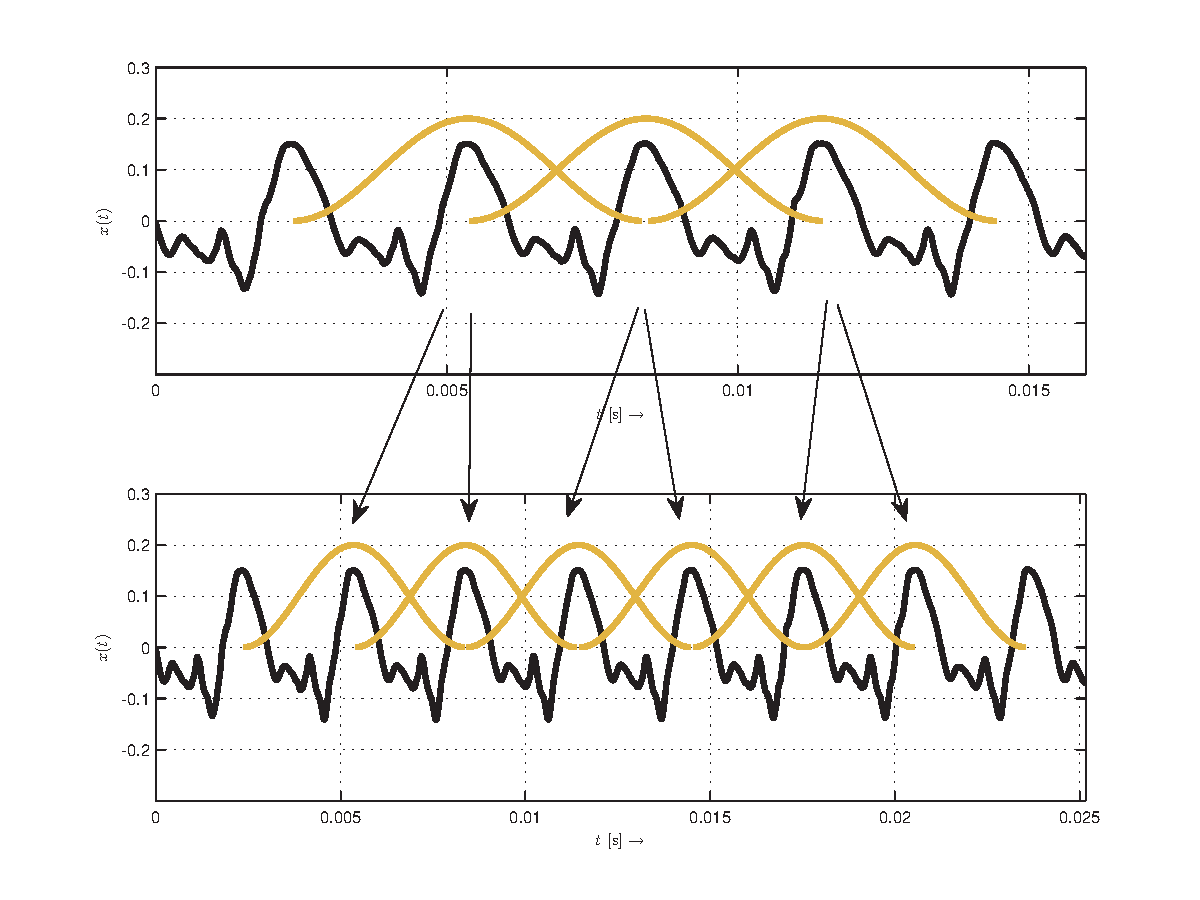
\includegraphics[scale=.3]{graph/PSOLA.pdf}
                    \end{figure}\vspace{-5mm}

                \column{4cm}\vspace{-20mm}
                    \begin{itemize}
                        \item orig  \includeaudio{audio/cathy.mp3}
                        \item $s = \nicefrac{4}{3}$ \includeaudio{audio/cathySOLout.mp3}
                    \end{itemize}
            \end{columns}
            \vspace{50mm}
    \end{frame}
\begin{frame}{PSOLA}\framesubtitle{transient copying}
				\begin{figure}
					\centerline{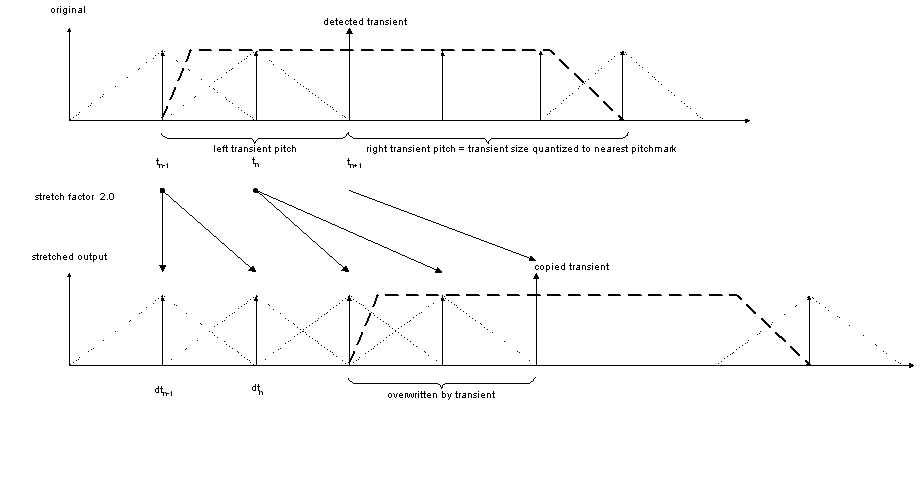
\includegraphics[scale=.3]{graph/transcpy}}
				\end{figure}
\end{frame}

    \begin{frame}{PSOLA}{time stretching summary}
        \begin{itemize}
            \item   \textbf{processing steps}
                \begin{enumerate}
                    \item   detect \textit{fundamental frequency}/period length
                    \item   set \textit{pitch marks}
                    \item   intelligently \textit{select blocks} to be repeated/discarded
                \end{enumerate}
            \pause
            \item   \textbf{advantages}
                \begin{itemize}
                    \item   \textit{high granularity} --- modify audio on period length resolution
                    \item   \textit{high quality}
                \end{itemize}
            \pause
            \item   \textbf{problems}
                \begin{itemize}
                    \item   quality depends on \textit{pitch tracking} reliability
                    \item   quality and timbre depends on \textit{pitch mark positioning}
                    \item   works only for \textit{monophonic} input signals
                        \begin{itemize}
                            \item   polyphonic and noisy segments
                            \item reverberation and overlapping tones
                        \end{itemize}
                   \item    \textit{noise, plosives} require special consideration
                   \item    \textit{copying} artifacts (double transients, timing deviations)
                \end{itemize}
            \pause
            \item   \textbf{typical applications}
                \begin{itemize}
                    \item   \textbf{standard approach for vocal editing tools}
                \end{itemize}
        \end{itemize}
    \end{frame}
